\documentclass[a4paper]{article}
\usepackage{todonotes}
\usepackage{amsmath}

\usepackage{listings}
\usepackage{color}
\usepackage{enumerate}

%Colors for the listings
\definecolor{dkgreen}{rgb}{0,0.6,0}
\definecolor{gray}{rgb}{0.5,0.5,0.5}
\definecolor{mauve}{rgb}{0.58,0,0.82}
%style setup for the listings
\lstset{frame=tb,
  language=Eiffel,
  aboveskip=3mm,
  belowskip=3mm,
  showstringspaces=false,
  columns=flexible,
  basicstyle={\small\ttfamily},
  numbers=none,
  numberstyle=\tiny\color{gray},
  keywordstyle=\color{blue},
  commentstyle=\color{dkgreen},
  stringstyle=\color{blue},
  breaklines=true,
  breakatwhitespace=true
  tabsize=3
}

\newcommand{\inline}[1]{\lstinline!#1!}%Inline code


\begin{document}

\section{Introduction}
\subsection{Basic definitions}
\begin{itemize}
\item Class: A class is a description of a possible set of run-time objects. It only exists in the software text.
\item Object: 
\begin{itemize}
\item An object is a software machine that allows program elements to access and modify a collection of data.
\item  It's an actual representation (instance) of a class (generating class). 
\item Objects only exist at runt-time and are visible in the program text through names.
\end{itemize}\item Feature: An operation that may be applied to all the objects of a class.
\begin{itemize}
\item Command: 
\begin{itemize}
\item No return value
\item Does modify the state of the objects
\item On the syntactical level, it is an instruction. 
\item May or may not have arguments
\end{itemize}
\item Query: 
\begin{itemize}
\item Returns a value
\item Does not modify the state of any object
\item The syntax equivalent is the expression.
\item May or may not have arguments
\item Functions get their results through computation
\item Attributes are values directly stored in memory
\end{itemize}
For queries, there is the uniform access principle, which states that it doesn't matter to the client whether a query is implemented as a function or attribute. Features should be accessible to clients the same way whether implemented by storage or by computation.
\item Creation Procedure: Commands to initiate objects, can be several. There is also a \inline{default_create}, which is inherited by all classes, and does nothing by default. 
\end{itemize}
\begin{center}
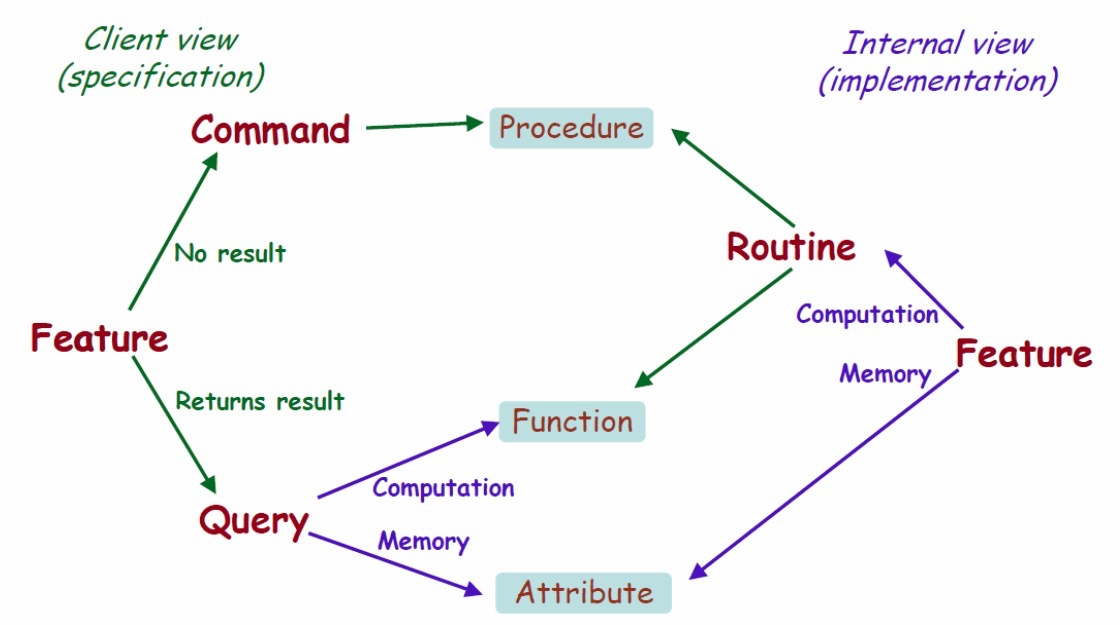
\includegraphics[scale=0.25]{Figures/featureQuery.jpg}
\end{center}
\item Feature Calls
\begin{itemize}
\item Unqualified calls: Feature calls which apply to the current object, e.g. \inline{f(args)}. Has \inline{Current} as an implicit target.
\item Qualified calls: Feature calls which apply to a certain object (has an explicit target), causing this object to become the current object, e.g. \inline{x.f(args)}
\end{itemize}
\item Class clauses
\begin{itemize}
\item Indexing
\item Inheritance
\item Creation
\item Feature
\item Invariant
\end{itemize}
\item Specimen: A syntactic element, such as a class name or an instruction, but no delimiters. The type of a specimen is its construct. See Describing syntax in the book.
\item Abstract syntax tree: Shows the syntax structure with all its specimens, but obviously without any delimiters, A tree has nodes, each one of the following kind:
\begin{itemize}
\item Root: Node with no incoming branch.
\item Leaf: Node without outgoing branches
\item Internal node: Neither of the former
\end{itemize}
\item Basic elements of a program text:
\begin{itemize}
\item Terminals
\begin{itemize}
\item Identifiers: Names chosen by the programmer
\item Keywords
\item Special symbols, such as a period
\end{itemize}
\end{itemize}
\item Describing a program
\begin{itemize}
\item Semantic rules: Define the effect of programming, satisfying the syntax rules
\item Syntax rules: Define how to make up specimens out of tokens satisfying the lexical rules
\item Lexical rules: Define how to make up tokens out of characters
\end{itemize}
\item Syntax: The way you write a program; characters grouped into words, grouped into bigger structures. 
\item Semantics: The effect you expect from this program at runtime
\item Identifier: Name chosen by the programmer to represent certain program elements, such as classes, features or runtime values. If it denotes a runtime value, it is called an identity or variable if it can change its value. During execution, an entity may become attached to an object. 
\item Creating an object consists in:
\begin{itemize}
\item If a class has no \inline{create} clause, use basic form: \inline{create x}
\item If the class has a \inline{create} clause listing one or more procedures, use \inline{create x.make()}, where \inline{make()} is one of the creation procedures, and \inline{(...)} stands for the arguments
\end{itemize}
\end{itemize}



\subsection{Variables}
\begin{itemize}
\item Types
\begin{itemize}
\item Reference types: 
\begin{itemize}
\item Entities with a reference value (contains the address, which can be the reference or location of the object).
\item They don't exist when we declare them (they are initially \inline{void}), like so: \inline{s: STATION}
\item We need to explicitly create them with a create instruction (\inline{create s})
\end{itemize}
\item Expanded types:
\begin{itemize}
\item Entities with an object as a value (points directly to the object)
\item They exist by just declaring them (they are never \inline{void})
\item Entities of expanded types are compared by value!
\item To declare an expanded type:
\begin{lstlisting}
expanded class COUPLE
feature --Access
	man, woman: HUMAN
	years_together: INTEGER
end
\end{lstlisting}
All entities of type \inline{COUPLE} will automatically become expanded, i.e. \inline{pitt_and_jolie: COUPLE}
\item Default values:
\begin{itemize}
\item \inline{false} for \inline{BOOLEAN}
\item 0 for numeric types (\inline{INTEGER}, \inline{NATURAL}, \inline{REAL})
\item ``null'' for \inline{CHARACTER}
\end{itemize}
\end{itemize}
\item A type is one of:
\begin{itemize}
\item A non-generic class
\item A generic derivation, i.e. the name of a class followed by a list of types, the actual generic parameters, in brackets
\end{itemize}
\end{itemize}
\item Setters: It is possible to make assignments such as \inline{x.att:=val}, which is shorthand for \inline{x.set_att(val)}
\item Effect of an assignment
\begin{itemize}
\item Reference types: Reference assignment
\item Expanded types: Value copy
\end{itemize}
\item Variable copy
\begin{itemize}
\item Shallow object duplication (creates a new object): \inline{b:=a.twin}
\item Deep object duplication (creates a new object): \inline{b:=a.deep_twin}
\item Shallow field-by-field copy (does not create an object): \inline{b.copy(a)}
\end{itemize}
\end{itemize}
\begin{center}
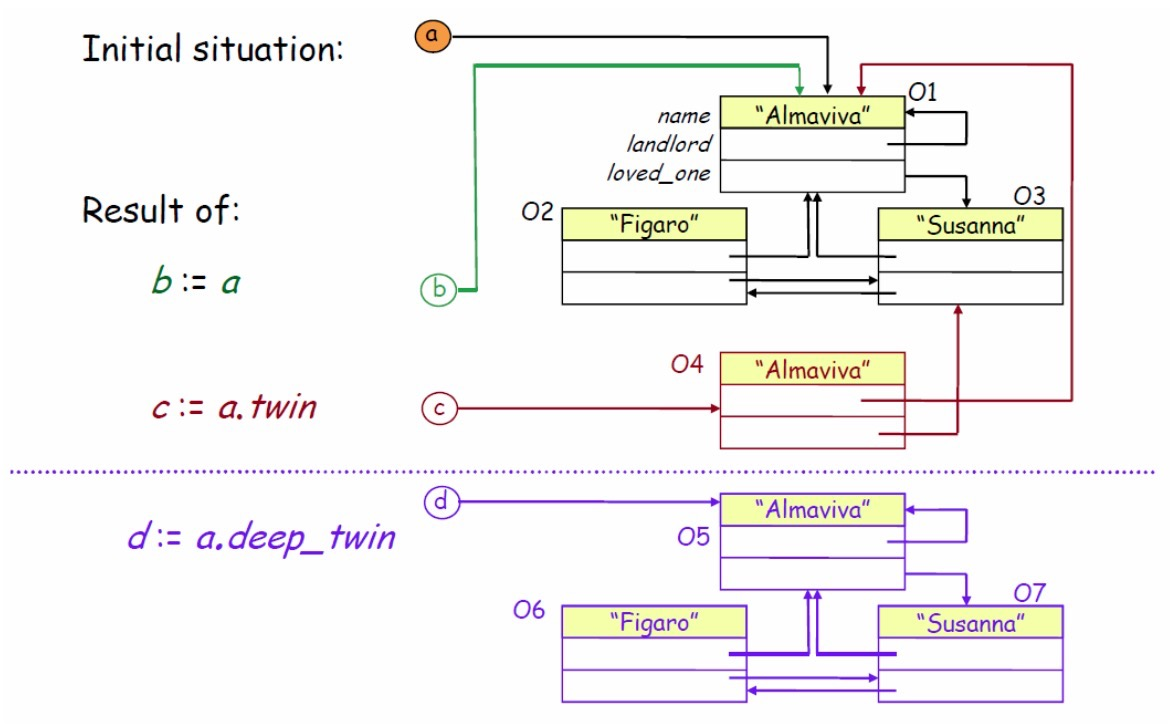
\includegraphics[scale=0.27]{Figures/variableCopy.jpg}
\end{center}
\subsection{Interface}
\begin{itemize}
\item A client of a software mechanism is a system of any kind - such as a software element or a human - that uses it. For its client, the mechanism is a supplier
\item The client is interested in a set of services that a software module provides, not its internal representation (what not how)
\item Interface: The description of techniques enabling clients to use these mechanisms. For example: GUIs (Graphical User Interface), command line interfaces (shell, bash,\dots), or APIs
\item An object can be an instance of a class, if the class is the generating class of the object
\end{itemize}

\subsection{Information Hiding}
\begin{itemize}
\item For its clients, an attribute may be:
\begin{itemize}
\item Secret
\item Read-only
\item Read, but partially write restricted (only certain things are allowed to be written)
\item Writing one or more classes in curly brackets after the keyword \inline{feature} exports these 
features only to these classes and its descendants. If no class is listed, the features 
are exported to \inline{ANY}. 
\end{itemize}
Information hiding only applies to use by clients using dot or infix notation. Unqualified calls are not subject to information hiding. 
\end{itemize}

\subsection{Control structures}
\begin{itemize}
\item Sequence or compound: consists of instructions listed in a certain order. Its execution consists of executing these instructions in the same order
\item Loop: consists of a sequence of instructions to be executed repeatedly.
\begin{lstlisting}
from
	--initialization Instructions
invariant
	--Loop invariant: Must hold true, satisfied after initialization, after the from clause
until
	--Exit condition; the condition under which the loop stops
loop
	--Instructions to be executed in each of the successive iterations
variant
	--Non-negative, decreases after every iteration
end
\end{lstlisting}
\begin{itemize}
\item Loop invariant
\begin{itemize}
\item Satisfied \textbf{after} initialization, after the \textsl{from} clause
\item Preserved by every loop iteration executed with the exit condition not satisfied. So in the end, the loop invariant \underline{and} the exit condition hold!
\end{itemize}
\item Loop variant
\begin{itemize}
\item Non-negative (i.e. $\geq$ 0) integer expression, right after initialization
\item Decreases while remaining non-negative for every iteration of the body with exit condition not satisfied. 
\item A loop with a correct variant cannot be infinite
\end{itemize}
\end{itemize}
\item Conditional: consists of a condition and two sequences of instructions. Its execution consists of executing one or the other of these sequences depending on whether the condition evaluates to \inline{true} or \inline{false}.
\begin{lstlisting}
if condition then
	-- Do something
elseif condition_2 then
	-- Do something different
else
	-- Do something else
end
\end{lstlisting}
\end{itemize}

\subsection{Contracts}
\begin{itemize}
\item Contracts are made of assertions, each containing an assertion tag and a condition (a Boolean expression), i.e. \inline{not_too_small: i>=1}
\item Precondition
\begin{itemize}
\item Property that a feature imposes on every client
\item If there is no \inline{require} clause, the precondition always evaluates to \inline{true}, as if it was written like this:
\begin{lstlisting}
require
	always_OK: true
\end{lstlisting}
\end{itemize}
\item Postcondition
\begin{itemize}
\item Property that a feature guarantees on termination to every client
\item A feature with no \inline{ensure} clause always satisfies its postcondition, as if it was written like this:
\begin{lstlisting}
ensure
	always_OK: true
\end{lstlisting}
\item Can make use of keyword \inline{old} (checks the result against the previous value of it)
\end{itemize}
\item Class invariant
\begin{itemize}
\item The invariant expresses consistency requirements between queries of a class
\end{itemize}
\end{itemize}

\subsection{Miscellaneous}
\begin{itemize}
\item Semistrict operators
\begin{itemize}
\item Lets us define the order of expression evaluation:
\begin{itemize}
\item \textbf{and then} is the semistrict version of \textbf{and}. Use it if a condition only makes sense when another is true.
\item \textbf{or else} is the semistrict version of \textbf{or}. Use it if a condition only makes sense when another is false
\item\textbf{implies} is always semistrict!
\end{itemize}
\end{itemize}
\end{itemize}

\section{Describing syntax}
\subsection{BNF}
Backus-Naur-Form (BNF): A metasyntax used to express context-free grammars. A formal way to describe formal languages. It consists of the following parts
\begin{itemize}
\item \textbf{Delimiters}: Fixed tokens of the languages vocabulary, such as keywords and special symbols
\item \textbf{Constructs}: They represent structures of the language, for instance \emph{Conditional}. A particular instance of a construct or known as a specimen of the construct. There are two kinds of constructs:
\begin{itemize}
\item \textbf{Nonterminal construct}: They are defined by a production
\item \textbf{Terminal construct}: Terminal constructs such as \emph{Identifier} or \emph{Integer} are not defined by this grammar, they are described at the lexical level
\end{itemize}
\item \textbf{Productions}: They are associated with a particular construct and specify their specimens
\end{itemize}
Each production defines the syntax of specimens of a particular construct, in terms of other constructs and delimiters. An example for a production (not BNF-E) 
\[A=B|C[D]\{ E``;''\}^*\]
Depending on the right side of a production, they can be separated into three kinds:
\begin{itemize}
\item \textbf{Concatenation}: This production lists zero or more constructs, some may enclosed in brackets and said to be \textbf{optional}
\item\textbf{Choice}: Listing one or more constructs, separated by vertical bars. A choice specifies that every specimen of the construct on the left consists of exactly one specimen of one of the constructs on the right
\item \textbf{Repetition}: A construct, enclosed in curly brackets, followed by a star. This indicates zero or more occurrences of the construct, Example: $A=\{ B\}^*$. The star might be replaced by a plus, indicating one or more repetition
\end{itemize}
\subsection{BNF-E}
\begin{itemize}
\item Every non-terminal must appear on the left side of exactly one production, called its defining production. 
\item Every production must be of one kind: either concatenation, choice or repetition
\item There is also a major change in the repetition production. Instead of \[A=[B \{\text{terminal }B\}^*]\] one may write \[A=\{B\text{ terminal }\dots\}^*\] The same is also true for the plus instead of a star.
\end{itemize}

\subsection{Regular Grammar}
The regular grammar is generally used to describe the terminal construct, which could be done using BNF, but can be achieved more easily using a regular grammar. The rules are quite similar, although different:
\begin{itemize}
\item The use of \textbf{choice} is no problem, possibly with character intervals
\item There are also \textbf{concatenations}, although they do not assume breaks (spaces, new lines, \dots) between elements. But you may define them explicitly using a lexical construct.
\item \textbf{Repetitions} have a different, simpler form; $A^*$ or $A^+$, following the same rules
\item No \textbf{recursion} is allowed whatsoever. As a result you may write any language in a single regular expression
\item Unlike BNF-E, you may mix different kinds of productions 
\end{itemize}

\section{Inheritance and Genericity}
\subsection{Inheritance}
\begin{itemize}
\item Principle: Describe a new class as extension or specialization of an existing class (or several with multiple inheritance)
\item If \inline{B} inherits from \inline{A}:
\begin{itemize}
\item As modules: All the services of \inline{A} are available in \inline{B} (possibly with a different implementation)
\item As types: Whenever an instance of \inline{A} is required, an instance of \inline{B} will be acceptable
\end{itemize}
\item Deferred classes:
\begin{itemize}
\item Deferred classes can have deferred features
\item A class with at least one deferred feature must be declared as deferred
\item A deferred feature does not have an implementation yet
\item Deferred clauses cannot be instantiated and hence cannot contain a create clause
\end{itemize}
\item Effective classes:
\begin{itemize}
\item Effective classes do not have deferred features
\item Effective routines have an implementation of their feature body
\end{itemize}
\item Terminology
\begin{itemize}
\item A class is a \textbf{parent} to another, if the other inherits directly from it, i.e. class \inline{A} is a parent to class \inline{B}, if class \inline{B} inherits from class \inline{A}
\item The \textbf{descendants} of a class are the class itself and (recursively) the descendants of its heirs (parents). \textbf{Proper descendant} excludes the class itself.
\end{itemize}
\begin{center}
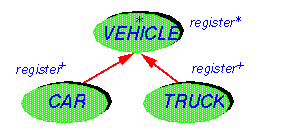
\includegraphics[scale=1]{Figures/inheritance_example.png}
\end{center}
\item \textbf{Features of classes}
\begin{itemize}
\item They can be \textbf{inherited} if it is a feature of one of the parents of the class. They can also be \textbf{immediate} if it is declared in the class. In this case, the class is said to introduce the feature
\item Fully implemented features are called \textbf{effective}, otherwise one may call them \textbf{deferred}
\end{itemize}
\item Contracts 
\begin{itemize}
\item The \textbf{invariant} of a class automatically includes the invariant clause from all its parents, and-ed
\item If no pre-/post condition is explicitly stated, features inherit the contracts from their parents
\item One can weaken the precondition with the keyword \inline{require else}, resulting in a precondition \inline{orig_pre} and \inline{new_pre}
\item One can strengthen the postcondition with the keyword \inline{ensure then}, resulting in a postcondition \inline{orig_post} and \inline{new_post}
\end{itemize}
\end{itemize}

\subsubsection{Multiple Inheritance}
\begin{itemize}
\item \textbf{Name clash}: If \inline{C} inherits both from \inline{A} and \inline{B}, which both have a feature \inline{f}, then we have a name clash. To resolve it, we can redefine one feature as \inline{A_f}. A name clash must be resolved, unless:
\begin{itemize}
\item It is under repeated inheritance (the feature of \inline{f} in \inline{A} and \inline{B} comes from a common ancestor, for instance \inline{ANY})
\item If at most one of the features \inline{f} is effective, and all others are deferred. In that case (only one feature is effective), the features are said to be \textbf{merged}. Merging also works when one or more features are renamed. The merging happens after renaming!
\item If more than one feature are effective, merging can still help. We can \textbf{undefine} effective features, so that they are deferred again. Syntax: \inline{undefine a,b,c end}. It is even possible to first rename a feature, undefine it and then merge it. 
\item They all have the same signature
\end{itemize}
\item Repeated Inheritance
\begin{itemize}
\item Features, not renamed along any of the inheritance paths, will be shared
\item Features, inherited under different names will be replicated
\item A potential ambiguity arises because of polymorphism and dynamic binding when class \inline{C} inherits from \inline{B} and \inline{A}, but \inline{A} redefines now copy (a feature of the common ancestor \inline{ANY}). In this case, a simple rename will not be enough, we have to select (\inline{select copy, f end}) the features from one parent, and rename the ones from the other.
\end{itemize}
\end{itemize}

\subsection{Genericity}
\begin{itemize}
\item Terminology:
\begin{itemize}
\item A \textbf{formal generic parameter} is the parameter in the class, e.g. \inline{LIST[G]} with \inline{G} as formal generic parameter.
\item An \textbf{actual generic parameter} is the actual type passed as parameter in a type, e.g. \inline{LIST[INTEGER]} with \inline{INTEGER} being the actual generic parameter. 
\item One can obtain a \textbf{generic derivation} of a generic class by passing a type
\end{itemize}
\item Static vs. Dynamic types:
\begin{itemize}
\item Static types are the types that we use while writing, to declare types for entities (arguments, locals, return values)
\item Dynamic types are created at run-time. Whenever an object is created, it gets assigned to be of some type. 
\end{itemize}
\item Types
\begin{itemize}
\item \textbf{Unconstrained} genericity: Any generic type is allowed. Example: \inline{LIST[G]}, which is the same as \inline{LIST[G->ANY]}
\item \textbf{Constrained} genericity: Only descendants are allowed as generic type. Example: \inline{LIST[G->NUMERIC]}
\end{itemize}
\end{itemize}

\subsection{Static Typing}
\begin{itemize}
\item \textbf{Type-safe call} (during execution). A feature call \inline{x.f} such that the object attached to \inline{x} has a feature corresponding to \inline{f}
\item \textbf{Static type checker} is a program-processing tool (such as a compiler) that guarantees for any program that it accepts, that any call in any execution will be type-safe
\item A programming language is called \textbf{statically typed language} if it is possible to write a static type checker
\end{itemize}

\subsection{Polymorphism}
\begin{itemize}
\item \textbf{Polymorphism} is the existence of the following possibilities:
\begin{itemize}
\item An \textbf{attachment} (assignment or argument passing) is \textbf{polymorphic} if its target variable and source expression have different types.
\item An entity or expression is polymorphic if it may at runtime, as a result of polymorphic attachments, become attached to objects of different types. 
\item A \textbf{container data structure} is polymorphic if it may contain references to objects of different types.  
\end{itemize}
\item The \textbf{static type} of an entity is the type used in its declaration in the class text. Similarly, the \textbf{dynamic type} of an entity is the type of the object, it is attached to. The type system ensures that the dynamic type of an entity will always conform to its static type.
\item \textbf{Conformance}
\begin{itemize}
\item A reference type \inline{U} \textbf{conforms} to a reference type \inline{T} if either:
\begin{itemize}
\item They have no generic parameters, and \inline{U} is a descendant of \inline{T}
\item They both are generic derivations with the same number of actual generic parameters, the base class of \inline{U} is a descendant of the base class of \inline{T}, and every actual parameter of \inline{U} (recursively) conforms to the corresponding actual parameter of \inline{T}
\end{itemize}
\item An expanded type only conforms to itself
\end{itemize}
\item \textbf{Object test}. Test the dynamic type of an object, e.g. \inline{if \{r:TYPE\} obj then ... end}
\begin{itemize}
\item \inline{ \{r:TYPE\} } is the object-test local, and only available in the \inline{then}-part, not in the \inline{else}-clause.
\item \inline{obj} is the object to be tested
\end{itemize}
\item \textbf{Assignment attempt}. Earlier mechanism for the object test. \inline{a?=b} assigns \inline{b} to \inline{a} if and only if \inline{b} is attached to an object whose type conforms to the type of \inline{a}. Otherwise, \inline{a} will be void
\end{itemize}

\subsection{Dynamic Binding}
\begin{itemize}
\item \textbf{Dynamic binding} as a semantic rule is the property that any execution of a feature call will use the version of the feature best adapted to the type of the target object.
\end{itemize}

\section{Recursion}
\begin{itemize}
\item \textbf{Definition}: A definition is recursive if it involves one or more instances of the concept itself. Recursion is the use of a recursive definition. 
\item Recursion can be either direct (routine \inline{r} calls \inline{r}) or indirect (routine \inline{r_1} calls \inline{r_2} .. calls \inline{r_n} calls \inline{r_1})
\item To be useful, a recursive definition should ensure that:
\begin{enumerate}[R1:]
\item There is at least one non-recursive branch
\item Every recursive branch occurs in a context that differs from the original
\item For every recursive branch, the change of context R2 brings it closer to at least one of the non-recursive cases R1
\end{enumerate}
\item Recursive calls cause (without further optimization) a run-time penalty: the stack of preserved calls needs to be maintained. Various optimizations are possible:
\begin{itemize}
\item Recursive schemes can sometimes be replaced by a loop (\textbf{recursive elimination})
\item \textbf{Tail recursion} (last instruction of a routine is a recursive call) can usually be eliminated 
\end{itemize}
\item \textbf{Recursive variant}: Every recursive routine should use a recursion variant, an integer quantity associated with any call, such that
\begin{itemize}
\item The variant is always $\geq 0$
\item If a routine execution starts with variant value $v$, the value $v'$ for any call satisfies $0\leq v'\leq v$
\end{itemize}
\end{itemize}

\section{Data Structures}
\subsection{Trees}
\subsubsection{Binary Trees}
\begin{itemize}
\item A binary tree \inline{G}, for an arbitrary data type \inline{G}, is a finite set of items called nodes, each containing a value of type \inline{G}, such that the nodes, if any, are divided into three disjoint parts:
\begin{itemize}
\item A single node, called the root of the binary tree
\item (Recursively) two binary trees over \inline{G}, called the left and right sub-tree
\end{itemize}
\item \textbf{Theorem:} For any node of a binary tree, there is a single downward path connecting the root to the node through successive applications of \inline{left} and \inline{right} links.
\item \textbf{Traversals}
\begin{itemize}
\item \textbf{In-order}: traverse left sub-tree, visit root, traverse right sub-tree
\item \textbf{Pre-order}: visit root, traverse left sub-tree, traverse right sub-tree
\item\textbf{Post-order}: traverse left sub-tree, traverse right sub-tree, visit root
\end{itemize}
\item \textbf{Binary search tree}: This is a tree over a sorted set \inline{G} if for every node \inline{n}:
\begin{itemize}
\item For every node \inline{x} of the left sub-tree of \inline{n}: \inline{x.item} $\leq$ \inline{n.item}
\item For every node \inline{x} of the right sub-tree of \inline{n}: \inline{x.item} $\geq$ \inline{n.item}
\end{itemize}
\item In a binary search tree, average behavior for insertion, deletion and search is $O\left( \log(n)\right)$, only worst case is $O(n)$
\end{itemize}

\begin{center}
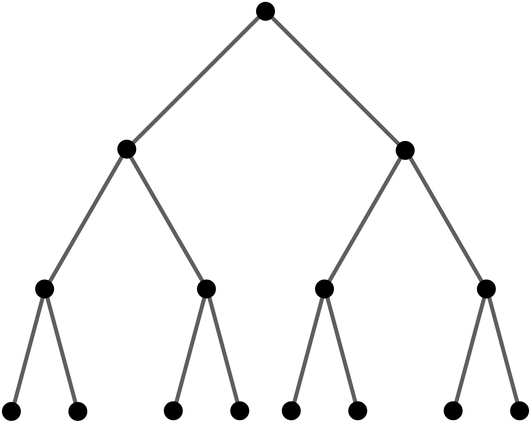
\includegraphics[scale=0.3]{Figures/rooted_binary_tree.png}
\end{center}

\subsection{Container data structures}
\begin{itemize}
\item Containers contain other objects, and store them in numerous ways. They differ in various properties, like the available operations, the speed of these operations and storage requirements. Some fundamental operations on a container:\\
\begin{center}
\begin{tabular}{|l|l|}
\hline
Insertion & Add an item\\\hline
Removal & Remove an occurence (if any) of an item\\\hline
Wipeout & Remove all occurences of an item\\\hline
Search & Find out if a given item is present \\\hline
Iteration (or trasversal) & Apply a given operation to every item\\\hline
\end{tabular}
\end{center}
\item The \inline{EiffelBase} classes use standard names for basic operations:
\begin{itemize}
\item Queries:
\begin{itemize}
\item \inline{is_empty: BOOLEAN}
\item\inline{has(v:G): BOOLEAN}
\item \inline{count: INTEGER}
\item \inline{item: G}
\end{itemize}
\item Commands
\begin{itemize}
\item \inline{make}
\item \inline{put(v:G)}
\item\inline{remove(v:G)}
\item\inline{wipe_out}
\item\inline{start, finish}
\item\inline{forth, back}
\end{itemize}
\end{itemize}
\item The \textbf{cursor} is present in many containers. It ranges from $0$ to $count+1$, and \inline{before} and \inline{after} hold if the cursor is not on an item. In an empty list, the cursor is at position $0$
\item \textbf{Alias notation}. A feature may be declared as follows: \inline{item(i: INTEGER) alias "[]": G assign put}. It is then possible to do \inline{a[i]} for \inline{a.item(i)} and \inline{a.item(i) := x} or \inline{a[i] := x} for \inline{a.put(x,i)}
\end{itemize}
\subsubsection{Lists}
\begin{itemize}
\item A list is a sequence of elements of a certain type. List is a general concept and has various implementations, including \inline{LINKED_LIST}, \inline{TWO_WAY_LIST}, \inline{ARRAYED_LIST}, etc.
\item Lists have a \textbf{cursor}. The current cursor position can be obtained by the query \inline{index}. The element at this position is generally obtained by \inline{item} and there are many other queries about the cursor position: \inline{after}, \inline{before}, \inline{off}, \inline{is_first}, \inline{is_last}
\item There are also various commands for \textbf{cursor movement}: \inline{start}, \inline{finish}, \inline{forth}, \inline{back}, \inline{go_i_th}
\item \textbf{Adding and removing} elements is done using: \inline{put_front}, \inline{put_left}, \inline{put_right}, \inline{extend}, \inline{remove} (item at cursor position)
\end{itemize}
\subsubsection{Arrays}
\begin{itemize}
\item An array is characterized by:
\begin{itemize}
\item Constant time for random reads/writes
\item Costly to resize (including inserting elements in the middle of the array)
\item Must be indexed by an integer
\item Generally very space efficient
\end{itemize}
\item Even though arrays are of fixed size with a capacity of \inline{upper-lower+1}, they can be resized. Instead of \inline{put} you may use \inline{force}, which has no precondition and resizes the array when needed.
\end{itemize}
\subsubsection{Hash Tables}
\begin{itemize}
\item Both arrays and hash tables are indexed based structures: Item manipulation requires an index, or, in case of  hash tables, a key. 
\item Unlike arrays, table allow keys other than integers: \inline{HASH_TABLE[ITEM_TYPE, KEY_TYPE->HASHABLE]}
\item Hash tables depend on hash functions, which map $K$, the set of possible keys, into an integer interval $a\dots b$. A perfect hash function gives a different integer value for every element of $K$. Whenever two different keys give the same hash value, a collision occurs. 
\item In reality hash functions are never perfect, so we need to deal with collisions. The following approaches deal with the problem:
\begin{itemize}
\item \textbf{Open hashing}: The data structure for this strategy is \inline{ARRAY[LINKED_LIST[G]]}. In each entry of the array, for a certain index $l$, you find the list of objects whose keys hash to $i$. The costs of search are $O(1)$ to find the correct array index by hashing the key and $O(c)$ to find the item in the linked list. $c$ is therefore a collision factor. With constant capacity of our array, the costs will become $O(\mathrm{count}/\mathrm{capacity})$, so this approach is somehow limited
\item \textbf{Closed hashing} (used by \inline{HASH_TABLE}): Here we have a single \inline{ARRAY[G]} where at any time some of its positions are occupied and some free. If for an insertion the hash function yields an already occupied position, the mechanism will try a succession of other positions until it finds a free one.\\
A common technique, of the hash function yields a first candidate position \inline{i=f(key) mod capacity}, is to try successive positions \inline{i+k*increment}, where increment is \inline{f(key) mod (capacity+1)}.\\
These are remarkably good results, since search with a good hash function becomes essentially $O(1)$
\end{itemize}
\end{itemize}

\subsubsection{Tuples}
\begin{itemize}
\item In mathematics, computer science, linguistics, and philosophy a tuple is an ordered list of elements. In set theory, an (ordered) $n-$tuple is a sequence (or ordered list) of elements, where $n$ is a non-negative integer
\item Tuples can be declared with
\begin{itemize}
\item Labeled arguments: \inline{TUPLE[INTEGER, STRING, PERSON]}
 \item Unlabeled arguments: \inline{tup: TUPLE[number: INTEGER, street: STRING, resident: PERSON]}
\end{itemize}
\item Is used like so:  \inline{tup := [99, "Weg", god_himself]}
\item One may think of tuples as of classes with only attributes. They therefore are also more interesting as a language mechanism to describe simple structures in a clear and simple way, rather than they are in the sense of a data structure.
\item Tags (like \inline{number} in the above example) are optional, they do not affect the type of a Tuple. 
\item A Tuple with no arguments can hold any tuple, one with only one argument may hold any tuples with at least one element with the first of same type, etc.
\item \textbf{Conformance}: You may assign an expression of type \inline{TUPLE[A,B,C]} to a variable of same type, or one of the following: \inline{TUPLE[A,B]} or \inline{TUPLE[A]} or \inline{TUPLE}
\end{itemize}

\subsubsection{Dispensers}
\begin{itemize}
\item These structures use no key or other identifying information for items, you insert an item just by itself. You also cannot choose what element you get by the query \inline{item}, Note: \inline{item} follows the command/query separation and therefore does not remove the item returned (you would need to make your own function, say \inline{get}). The policy used to determine which item to return, may be one of the following:
\begin{itemize}
\item \textbf{LIFO} (\textbf{L}ast \textbf{I}n, \textbf{F}irst \textbf{O}ut): Choose the element inserted most recently. Such dispenser is called a \textbf{stack}, and the stack operations are known as:
\begin{itemize}
\item \textbf{push}: Pushes an item to the top of the stack (command \inline{put})
\item \textbf{pop}: Pops the top item (command \inline{remove}). The body of a stack is what remains after popping
\end{itemize}
\item \textbf{FIFO} (\textbf{F}irst \textbf{In}, \textbf{F}irst \textbf{O}ut): Choose the oldest element not yet removed. Such dispenser is called \textbf{queue}.
\begin{itemize}
\item Queues do also have many applications, such as simulations (represent pending events) and GUI (handling user inputs)
\item As with stacks you may use arrayed or linked implementations. The linked one is straightforward, where the arrayed needs some special treatment. Because we always add new items at the end of the array and remove old ones from the beginning, at some point we will reach the end. Therefore, \inline{ARRAYED_QUEUE} is conceptually a ring.
\end{itemize}
\item With a \textbf{priority queue}, items have an associated priority.
\end{itemize}
\end{itemize}

\section{Agents}
\begin{itemize}
\item An object whose sole role is to describe an operation, for example if you want to treat an operation as an object
\item Every agent has an associated routine, which the agent wraps and is able to invoke.
\item To get an agent, use the \inline{agent} keyword, e.g. \inline{a_agent := agent my_routine}
\item Applications include:
\begin{itemize}
\item Iteration
\item Undoing (redo-undo)
\item Event-driven programming
\end{itemize}
\item The type of an agent is one of the following:
\begin{itemize}
\item \inline{PROCEDURE [BASE_TYPE, OPEN_ARGS -> TUPLE]}
\item \inline{FUNCTION [BASE_TYPE, OPEN_ARGS -> TUPLE, RESULT_TYPE]}
\item \inline{PREDICATE [BASE_TYPE, OPEN_ARGS -> TUPLE]}
\end{itemize}
\textbf{Note}: All these types inherit from the deferred class \inline{ROUTINE}, and \inline{PREDICATE} is furthermore a descendant of \inline{FUNCTION}
\item The important features of agents include \inline{call([open_args])}, and \inline{last_result}
\item \textbf{Open/closed arguments}: 
\begin{itemize}
\item An agent can have both ``closed'' and ``open'' arguments:
\begin{itemize}
\item \textbf{Closed arguments} are set at agent definition time
\item \textbf{Open arguments} are set at agent call time
\end{itemize}
\item To keep an argument open, replace it by a question mark, i.e. \inline{v := agent a0.f(a1,?,a3)}
\item All closed argument agent: \inline{u := agent a0.f(a1,a2,a3)}
\item If you omit the argument list, all arguments of the underlying function are considered open.
\end{itemize}
\item \textbf{Open target}: It is also possible to keep the target of an agent open, but then you need to specify its type. The target is then passed as first item in the argument tuple to the agent.
\item Here are some examples of agents:\\
\begin{tabular}{r l|l}
$-$ & \inline{u := agent {TARGET_TYPE}.f(?, ?, z)} & \inline{u.call([target,a,b])}\\
$-$ & \inline{u := agent a0.f(x, ?)} & \inline{u.call([a])}\\
$-$ & \inline{u := agent a0.f} & \inline{u.call([])}\\
$-$ & \inline{u := agent {TARGET_TYPE}.f} & \inline{u.call([target])}\\
\end{tabular}
\item Some example types:
\begin{itemize}
\item \inline{PROCEDURE[ANY, TUPLE]} (no open arguments)
\item \inline{PROCEDURE[ANY, TUPLE[X,Y,Z]]} (3 open args, with types \inline{X, Y, Z})
\item \inline{FUNCTION[ANY, TUPLE[X,Y],RES]} (2 open args, result of type \inline{RES})
\end{itemize}
\end{itemize}

\section{Event Driven Programming}
\subsection{Terminology}
\begin{itemize}
\item An \textbf{event} is a run-time operation, executed by a software element to make some information (including that it occurred) available for potential use by the software elements not specified by the operation. The information associated with an event (other than it actually occurred) constitutes the event's \textbf{arguments}
\item To \textbf{trigger} (or \textbf{publish}) an event is to execute it
\begin{itemize}
\item A software element that may trigger events is a \textbf{publisher}
\item A software element that may use the event's information is a \textbf{subscriber}
\end{itemize}
\item Any event belongs to an \textbf{event type}, and therefore shares the same argument list \textbf{signature}
\item Note: Event type/event may suggest corresponding to a type of OO programming, but in our model, an event is not an object! There is the \inline{EVENT_TYPE} in Eiffel, which denotes the \textbf{general idea} event types, and a particular event type is then an instance of this class.
\end{itemize}
\subsection{The event-driven scheme}
\begin{itemize}
\item Some elements, publishers, make known to the rest of the system what event types they may trigger
\item Some elements, subscribers, are interested in handling events of certain event types. They register the corresponding actions.
\item At any time, a publisher can trigger an event. This will cause execution of actions registered by subscribers for the event's type. These actions can use the event's arguments. 
\item In event-driven design, a \textbf{context} is a Boolean expression specified by  a subscriber at registration time, but evaluated at triggering time, such that the registered action will only be executed if the evaluation yields true. 
\end{itemize}

\subsection{Publish-Subscribe program}
In devising a software architecture supporting the publish-subscribe paradigm, we should consider the following requirements:
\begin{itemize}
\item Publishers must not need to know who the subscribers are
\item Any event triggered by one publisher may be consumed by several subscribers
\item The subscribers should not need to know about the publishers. \textbf{This goal cannot be provided by the observer pattern}
\item The subscribers can register and deregister while the application is running
\item It should be possible to make events dependent or not on a context
\item It should be possible to connect publishers and subscribers with minimal work
\end{itemize}
\subsubsection{Observer Pattern}
\begin{itemize}
\item Note that this pattern is limited, and therefore should not be used. Regardless the existence of superior methods, the observer pattern is still used very frequently.
\todo[inline]{Add observer pattern architecture picture}
\item \textbf{Publisher}: Describes the properties of a typical publisher in charge of an event type. It can trigger events through \inline{publish}, and subscribers can subscribe and unsubscribe
\item \textbf{Subscriber}:  on the other hand do also have subscribe and unsubscribe to (un-) subscribe to a 
particular publisher. The feature calls (un-)subscribe of the desired publisher, passing itself as 
argument. Furthermore there is the deferred feature handle which expects a \inline{LIST} as 
argument. This is not ideal, since there is no type safety with the \inline{LIST} as argument, but since 
the very general classes \inline{PUBLISHER} and \inline{SUBSCRIBER} need to know about the arguments, there is not really a better way. We could only specify the two classes further (e.g. one for 
each argument list), but therefore loosing generality. (Using genericity with tuples would 
work, but who does have them other than Eiffel? And Eiffel can do better..)
\item \textbf{Drawbacks} of the observer pattern:
\begin{itemize}
\item The argument business, see above
\item Subscribers subscribe directly to publishers rather than event types
\item A subscriber may register with only one publisher, with that publisher, it can register only one action
\item It is not possible to directly reuse an existing routine. The classes need to inherit from \inline{PUBLISHER}/\inline{SUBSCRIBER} resulting in too much glue code
\item The last problem gets even worse without multiple inheritance. 
\end{itemize}
\end{itemize}

\subsubsection{Event Type Library (A Much Better Approach)}
\begin{itemize}
\item There is only a single class \inline{EVENT_TYPE[ARGS -> TUPLE]} with a generic parameter, ensuring type safety. 
\item One can create event types, for instance:
\begin{lstlisting}
left_click: EVENT_TYPE[TUPLE[x:REAL,y:REAL]]
-- Event type representing left-button click events
	once
		create Result
	end
\end{lstlisting}
\item This declaration can take place in ``facilities'' class to which all others who need have access to (no context required). But it is also possible to put it in an ordinary class like \inline{BUTTON}, then having something like \inline{your_button.left_click.subscribe(agent p)} (context required)
\item To trigger an event, one may write: \inline{left_click.publish([your_x, your_y])}
\item To subscribe to an event, one may write: \inline{left_click.subscribe(agent p)}, requiring that \inline{p} represents a function with proper signature.
\end{itemize}
\end{document}